
\section{Cyclic processes}

\textcolor{violet}{Cyclic processes: thermodynamic process in which a system returns to its initial
	thermodynamic state (i.e same U, P. V. T) after a process.
	\begin{itemize}
		\item aka $\Delta U = 0$
	\end{itemize}
}
\begin{itemize}
	\item We are reminded of the first law: $\Delta U = \Delta Q - \Delta W$
	      \begin{itemize}
		      \item meaning for a cyclic process  $\rightarrow \Delta U = 0 \rightarrow Q = W$
		      \item total heat added over the cycle = total work done by the system
	      \end{itemize}
	\item Most of this section referenced Chapter 8 (Heat \& Work) from Kittel
\end{itemize}


\subsection{Energy \& Entropy Transfer Definitions}
\begin{itemize}
	\item \textcolor{violet}{heat is the transfer of energy to a system by thermal contact
		      with a reservoir}
	\item \textcolor{violet}{work is the transfer of energy to a system by a change in the
		      external parameters that describe the system}
	\item we want to convert heat to work (steam engine, combustion engine)
	\item bringing 2 systems together, the total energy is conserved but not the entropy,
	      may increase
	\item it is defined that $dQ \equiv T dS$ which means $dW = dU - dQ = dU - TdS$
	      \begin{itemize}
		      \item $dS = 0 \rightarrow$ pure work
		      \item $dU = TdS \rightarrow$ pure heat
	      \end{itemize}
\end{itemize}


\subsection{Heat Engines: conversion of heat into work}
\subsubsection{Carnot inequality}
\begin{itemize}
	\item all forms of work are freely convertible, they are thermodynamically
	      equivalent to each other
	\item work can be completely converted to heat but the inverse is not true
	      \begin{itemize}
		      \item entropy enters the system with the heat but does not leave the system with
		            the work
		      \item \textcolor{violet}{"To prevent the accumulation of entropy [in a system] there
			            must be some output heat; therefore it is impossible to convert all the input heat
			            to work!"}
		      \item entropy must ultimately be removed
	      \end{itemize}
	\item heat engine: energy conversion device that operates in cycles
	      \begin{figure}
		      \centering
		      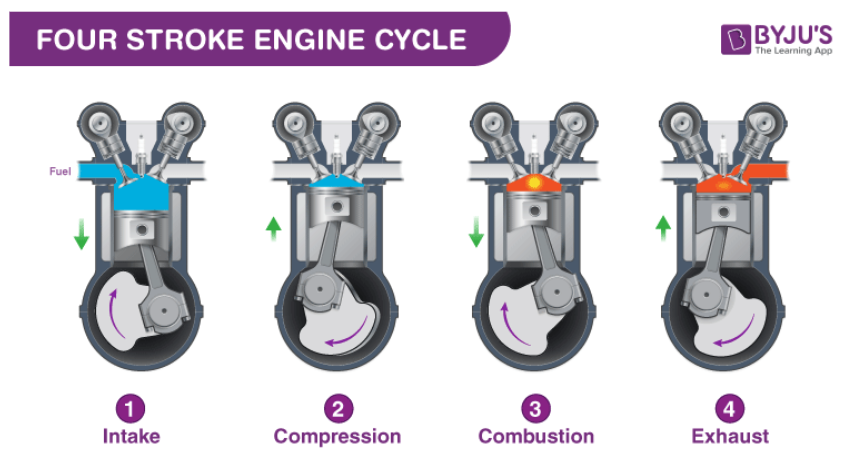
\includegraphics[width=.75\textwidth]{Figures/4StrokeEngineCycle.png}
		      \caption{Entropy is at the min near the beginning of the intake stroke and max at
			      the beginning of the exhaust stroke.}
		      \label{fig:engine_diagram}
	      \end{figure}
	\item work generated during 1 cycle of a reversible process:
	      \begin{align}
		      W = Q_h - Q_l = (1 - T_l/T_h)Q_h = \frac{T_h - T_l}{T_l} Q_h \\
		      \text{\textcolor{violet}{Carnot efficiency }} \eta_c \equiv (\frac{W}{Q_h})_\text{rev} = \frac{T_h - T_l}{T_l}
	      \end{align}
	      where h is the input heat and l is the leaving heat, \\
	      \textcolor{violet}{aka we can not convert all input heat into work}
	      \begin{align}
		      \text{Carnot inequality } \eta = W/Q \leq 1 - (T_l/T_h) \equiv \eta_c
	      \end{align}
	\item Carnot inequality is the basic limit for heat engines
\end{itemize}


\subsubsection{Refrigerators}
\begin{itemize}
	\item refrigerators consume work to remove heat
	      \begin{align}
		      \text{coefficient of refrigerator performance } \lambda \equiv Q_l /W
	      \end{align}
	      $\lambda$ can be greater or less than 1
	      \begin{align}
		      \text{Carnot coefficient of refrigerator performance } \lambda_c = (Q_l/W)_\text{rev} = \frac{T_l}{T_h - T_l}
	      \end{align}
	      This is an upper limit to the actual coefficient of refrigerator
	\item air conditioners are refrigerators
	\item heat pumps are reverse connections of an air conditioner
\end{itemize}


\subsubsection{Carnot Cycle}
\begin{itemize}
	\item gas is expanded \& compressed in 4 stages (2 isothermal \& 2 isentropic)
	      \begin{enumerate}
		      \item gas has the temp $T_\text{high}$ \& entropy $S_\text{Low}$
		            \begin{itemize}
			            \item gas expands at constant T until the entropy increases to $S_H$
		            \end{itemize}
		      \item gas has the temp $T_h$ \& entropy $S_H$
		            \begin{itemize}
			            \item gas expands with constant S, until temp drops to $T_l$
		            \end{itemize}
		      \item gas has the temp $T_l$ \& entropy $S_H$
		            \begin{itemize}
			            \item gas is compressed isothermally
		            \end{itemize}
		      \item gas has the temp $T_l$ \& entropy $S_L$
		            \begin{itemize}
			            \item compressed isentropically to original state
		            \end{itemize}
	      \end{enumerate}
	\item work done by the system is the area of the rectangle (Carnot cycle)
	      \begin{align}
		      W & = (T_h - T_l) (S_H - S_L) \\
	      \end{align}
	      which comes from
	      \begin{align}
		      \oint dU = 0 = \oint TdS - \oint pdV \rightarrow W = \oint TdS
	      \end{align}
\end{itemize}


\subsubsection{Path Dependence of Heat \& Work }
\begin{itemize}
	\item transfers of heat and work between state (a) and state (b) depend on the path
	      taken between the two states \textcolor{violet}{heat \& work are not state functions}
	\item "Without the path dependence of heat and work there would not exist cyclical
	      processes that permit the generation of work from heat."
\end{itemize}

\subsubsection{Irreversible Work}
\begin{itemize}
	\item if newly created entropy arises by the conversion of work to heat, irreversible
	      work has been performed
	\item pure heat transfer not involving any work done between 2 systems with different temperatures
\end{itemize}


\subsection{Heat \& Work at Constant Temp or Pressure }




end page 261!


\subsection{Some Discussion Notes}
\begin{itemize}
	\item reversible process
	      \begin{itemize}
		      \item to begin this system has no change in energy as well as entropy (like wut???)
		      \item since there is no change in entropy, it stands that there is no change in temp as:
		            \begin{align}
			            \Delta S_\text{tot} = \frac{-Q}{T_A} + \frac{Q}{T_B}
		            \end{align}
		            which means that there is no heat exchange
		      \item since $\Delta U = 0$ \& $\Delta Q = 0$ it stands that $\Delta W = 0$
		            ($\Delta U = \Delta Q - \Delta W$), \textcolor{violet}{aka no work is done!!}
		      \item this system is also quassi static which means it's always in equilibrium
	      \end{itemize}
\end{itemize}
